\newpage
\section{Of Angles and Circles} %%remove * if added to notes!

\fixnote{Fix to focus on arcs, not chords.  A chord defines two central angles and two arcs.  ``Standard'' and reflex angle pair.  Some of the claims below are true only for one of the arcs defined by the chord.}  

In this handout we are going to look at pictures and see if we can
explain how they ``prove'' theorems.


\begin{theorem} 
Any triangle inscribed in a circle having the diameter as a leg is a
right triangle.
\end{theorem}

\begin{prob}
Can you tell me in English what this theorem says? Provide some
examples of this theorem in action.
\end{prob}

\begin{prob} 
Here is a series of pictures, designed to be read from left to right.
\[
\includegraphics{../graphics/pbpcircthm1.pdf}
\]
Explain how these pictures ``prove'' the above theorem. In the process
of your explanation, you may need to label parts of the pictures and
do some algebra.
\end{prob}


\begin{theorem} 
Given a chord of a circle, the central angle defined by this chord is
twice any inscribed angle defined by this chord.
\end{theorem}

I'll play nice here and give you a picture of this theorem in action:
\[
\includegraphics[scale=0.8]{../graphics/pbpcircthm2eg.pdf}
\]

\begin{prob}
Can you tell me in English what this theorem says? For one thing, what
do the fancy words mean? Specifically, what is meant by
\textit{chord}, \textit{central angle}, and \textit{inscribed angle}?
\end{prob}

\begin{prob} 
For one possible line of reasoning, consider this series of pictures, designed to be read from left to right.
\[
\includegraphics{../graphics/pbpcircthm2.pdf}
\]

Explain how these pictures ``prove'' the above theorem. In the process
of your explanation, you may need to label parts of the pictures and
do some algebra.
\end{prob}

\fixnote{Need some teaching notes or help for the third figure below.  Two things that are hard:  adding the diameter (or other chord) and then seeing the overlapping angles.}
\begin{prob}
Sometimes it helps to organize the desired result into separate cases:  
% Can you show $m\angle AXB = \frac{1}{2}m\angle AOB$ for the sequence of cases below.  
\[
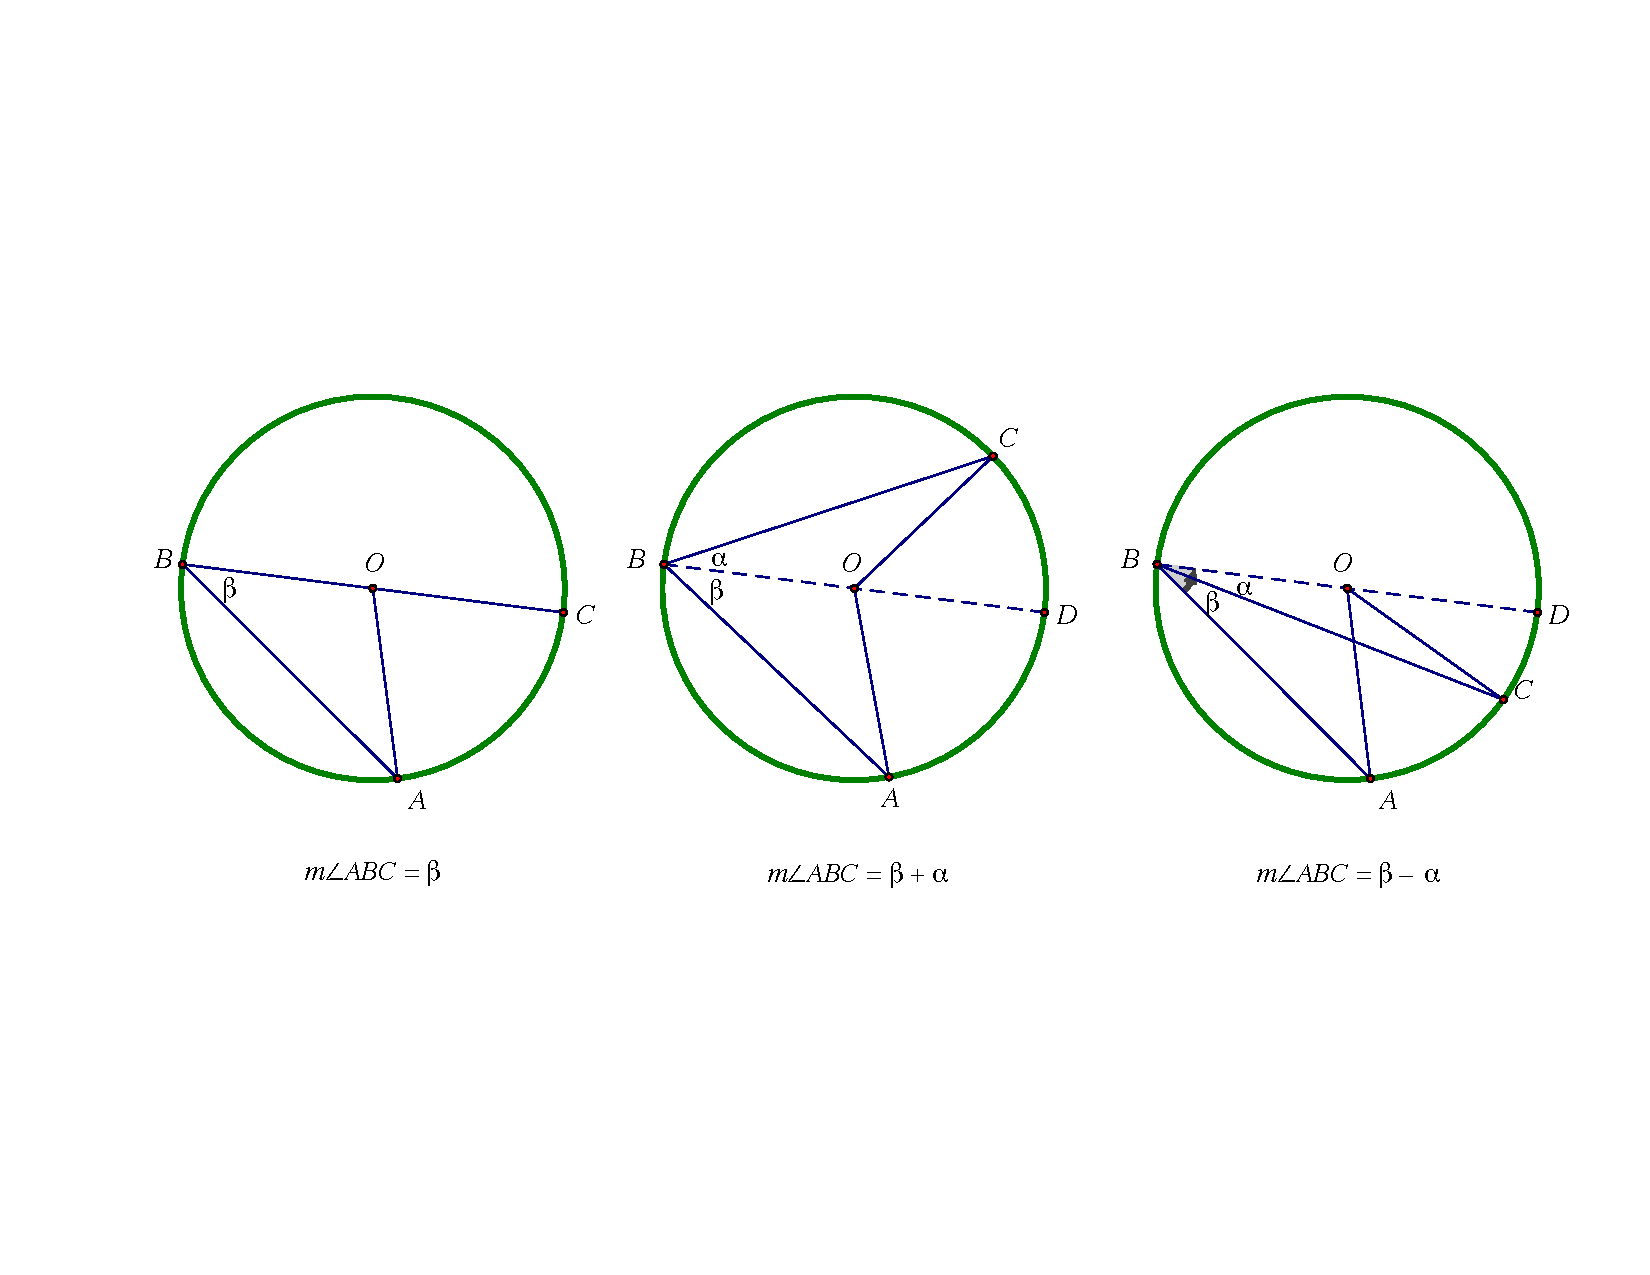
\includegraphics[width=3.5in]{../graphics/inscribedAngle.pdf}
\]
How do you need to modify the proof to be sure that you have handled all three cases?  
\end{prob}


\begin{corollary} 
Given a chord of a circle, all inscribed angles defined by this chord
are equal.
\end{corollary}

\begin{prob} 
Firstly---what the heck is a corollary? Secondly---what is it saying?
Thirdly---why is it true?
\end{prob}

